\begin{figure}[H]
  \centering
  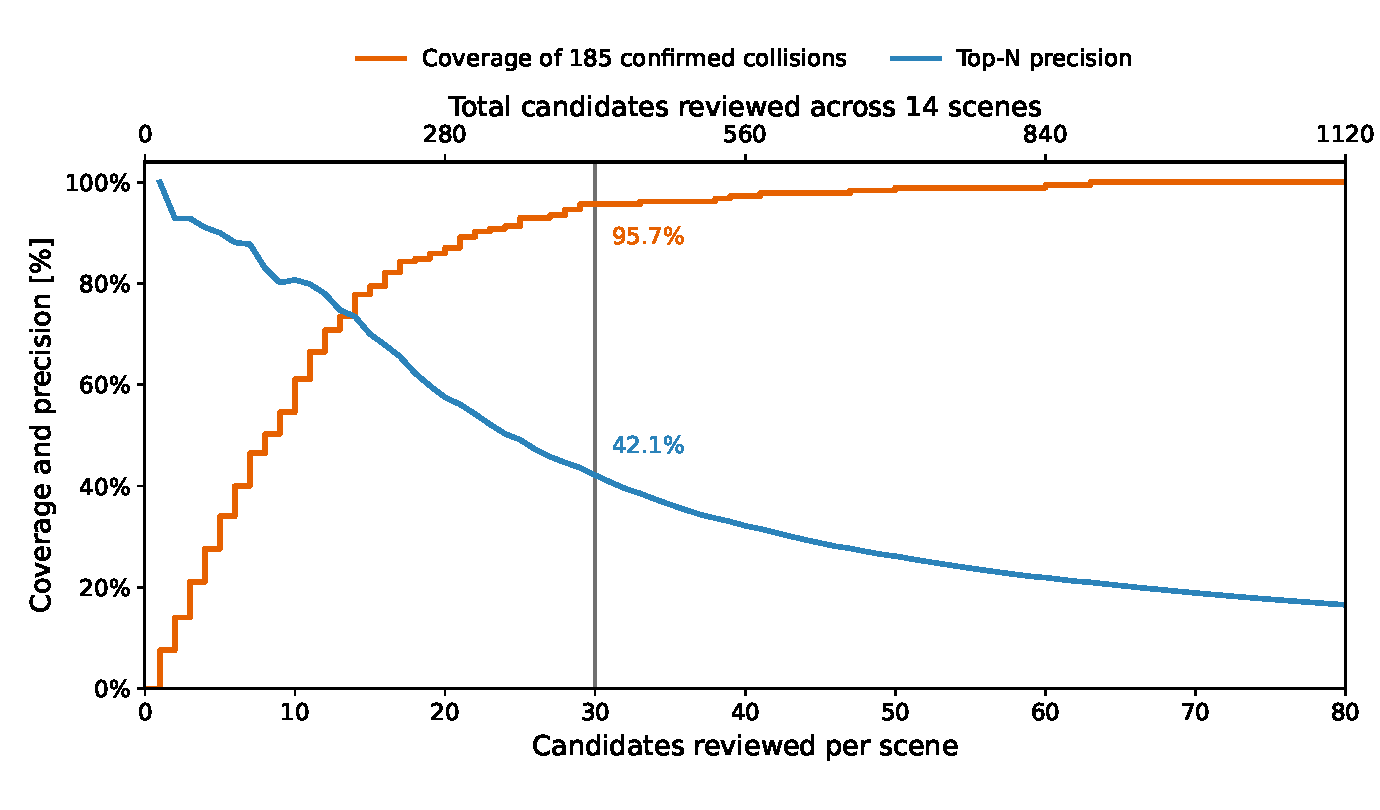
\includegraphics[width=\linewidth]{figures/expresult/review_budget_operating_points_260715.pdf}
  \caption{Coverage of confirmed events and review precision as functions of the number of candidates reviewed per experimental sequence. Candidates are reviewed in descending order of their final score within each of the 14 sequences. Coverage is the fraction of the 185 confirmed events recovered, whereas top-\(N\) precision is the fraction of reviewed candidates confirmed as events. The upper axis gives the total number reviewed across all sequences. Reviewing the top 30 candidates per sequence, or 420 candidates in total, recovers 177 events, corresponding to 95.7\% coverage and 42.1\% precision. Coverage is conditional on the confirmed-event set and is not an estimate of absolute experimental recall.}
  \label{fig:experimental_review_budget_operating_points}
\end{figure}
